\chapter{Design}
\label{cha:design}

This section describes the design of the file server, including both the interface through which clients interact with the system and the internal file system structure. As both components significantly influence how operations are issued and processed, their design plays a key role in overall system behaviour. 

\section{System Requirements and Constraints}

The design of the file server is driven by both functional requirements and the constraints imposed by Microkit and seL4. These requirements define the intended behaviour of the system, while the constraints shape the design decisions necessary to achieve this within the given environment.

From a functional perspective, the system is required to provide a core set of file system operations, including creation, reading, writing and deletion of files, alongside support for directory structures and getting and setting of associated metadata such as permissions and file size. The system must present a consistent and simple interface to clients, ensuring that operations are executed correctly and that appropriate error codes are returned in response to invalid inputs or failure conditions.

A key requirement of the system is support for multiple clients operating concurrently. The file server must therefore be capable of handling requests from multiple independent clients, maintaining correctness and consistency in the presence of interleaved operations. In addition, the system must support both synchronous and asynchronous interaction models. This will enable direct comparison between traditional blocking request–response behaviour and the proposed asynchronous, batched approach.

Performance is a central non-functional requirement. In particular, the system is designed to minimise the overhead associated with IPC, which is a known bottleneck in microkernel-based systems\cite{}. The asynchronous design must therefore enable efficient batching of operations, reducing the number of required IPC interactions and improving overall throughput. 

Several constraints significantly influence the system design. The Microkit framework enforces a statically defined system configuration to aid high-assurance and high-performance system development, meaning that all protection domains, communication channels and memory regions must be specified at build time. As a result, the number of clients and their associated resources are fixed, hindering the system's ability to adapt.

The IPC model provided by seL4 is inherently synchronous, with communication occurring through blocking interactions. This motivates the use of shared memory and notification mechanisms to enable non-blocking request submission and completion handling.

Hence, memory cannot be shared dynamically between protection domains, preventing the use of copy-free mechanisms that rely on on-demand sharing. Consequently, all data transfer must occur through these shared memory regions, requiring explicit buffer management within the interface design.

Further constraints arise from the execution environment. For development simplicity, the system operates with no access to persistent storage, resulting in a purely in-memory file system. Additionally, due to seL4 constraints, execution is limited to a single core, restricting the ability to exploit parallelism. This requires the system to rely on batching and efficient communication patterns, rather than parallel execution, to achieve performance improvements.

These requirements and constraints directly inform the design of the system, motivating the use of asynchronous batching, shared memory communication and a modular file system structure to balance performance, correctness and simplicity within the limitations of the Microkit environment.

\section{IPC Design and File Server Interface}

The file server interface defines how clients interact with the system to issue operations and receive results. As the interface determines how frequently and in what manner inter-process communication occurs, it plays a critical role in the overall performance of the system. Two models are considered: a synchronous interface, representing a traditional baseline for file server evaluation, and an asynchronous interface, designed to reduce communication overhead through batching and decoupling of request submission and processing. 

\subsection{Synchronous Model \textit{(Baseline)}}

This model represents a conventional microkernel interaction pattern, providing a simple and well-defined interface for issuing file system operations and receiving results.

The communication flow is as follows:
\begin{itemize}
    \item A client issues a single operation via a synchronous IPC call and blocks until the request is completed. 
    \item The server receives the request, processes the operation, and returns the result. 
    \item The client then resumes execution.
\end{itemize}

\newpage
This blocking behaviour enforces strict coupling between client and server execution. In this model, it is assumed any subsequent operation may depend on the result of the request, hence the client must do no further processing until the response is received. Consequently, client execution is effectively serialised with that of the file server, as shown in Figure \ref{fig:sync}, even if the client and server execute on different cores. Furthermore, the server itself only performs work when servicing requests and is otherwise idle.

As operations are strictly sequential, a single shared buffer per client is sufficient. Each request can reuse the same buffer, as its contents are consumed before the next operation is issued. This simplifies both memory management and interface design, as data is always read from and written to a consistent location.

To reduce overhead, non-data components of an operation may be passed directly within the IPC message. This avoids the need for complex parsing logic, as the shared buffer is reserved for file-related data such as filenames or read/write contents, while the IPC parameters encode the operation type and associated metadata, such as file descriptors or byte counts.

In a multiclient setting, blocking effects are amplified. If a client issues a request while the server is servicing another, it must wait not only for its own operation to complete but also for the server to become available, as shown in Figure \ref{fig:sync}. As a result, requests are effectively serialised across clients. Therefore, with more than 2 clients, the file server must maintain a queue of pending requests to ensure fair servicing, yet, this is bounded by the number of clients, limiting its complexity.

\begin{figure}[H]
    \centering
    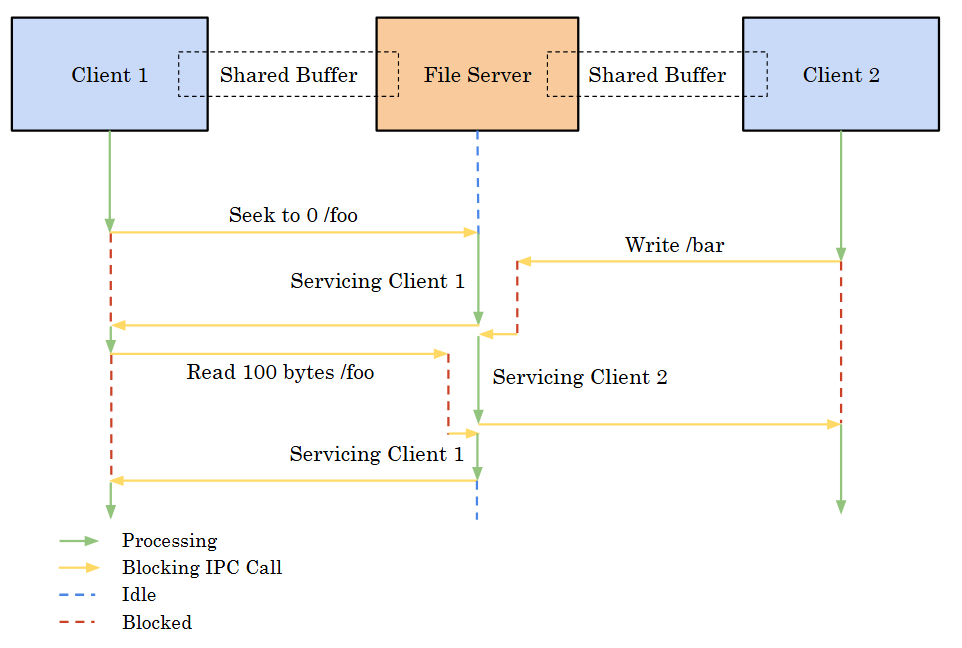
\includegraphics[width=0.6\linewidth]{chapters/images/sync.png}
    \caption{Synchronous multiclient-server interaction.}
    \label{fig:sync}
\end{figure}

Consequently, this model permits no concurrency in relation to the file server, and clients spend a significant portion of time blocked, particularly as the number of clients increases. Additionally, IPC overhead is incurred on a per-operation basis, as each request requires a dedicated interaction with the server. This makes it unsuitable for workloads where large numbers of independent operations are performed, but provides a clear and well-defined baseline for comparison with the asynchronous design.

\subsection{Asynchronous Model \textit{(Proposed IPC Mitigation Strategy)}}\label{sec:ipc_design}

The asynchronous model replaces the synchronous request–response interaction with a non-blocking, decoupled communication approach. While this increases the complexity of the interaction and the resources required, it enables significantly greater potential for performance improvement.

This non-blocking communication is achieved through a notification-based mechanism, rather than procedure calls. As a result, there is no requirement for a handshake or immediate response, allowing the client to issue a notification and continue execution without blocking, as illustrated by the continuous client execution in Figure~\ref{fig:async}. However, if the following computation relies upon the result of the requested operation, and no later processing may be moved forwards, the client will still have to wait. Yet, this model provides flexibility, enabling concurrency where possible while preserving correctness when dependencies exist.

When the server is idle, a notification triggers immediate processing of the corresponding request. Otherwise, unlike the synchronous system, where clients wait until the server becomes available to transfer their request, request submissions must be stored until they can be processed. As the server may be busy, this queuing cannot be managed internally by the server at the time of submission. Instead, each client is assigned a dedicated shared memory region with the server, used to queue outstanding requests. Notifications therefore carry no data, acting solely to signal that work is available, while the actual request data is retrieved by the server from these shared memory queues. As such, upon completing an operation the server polls these client queues to identify and service any pending requests that may have been submitted while it was busy.

To support efficient and correct operation, this shared memory must be carefully structured. As in the synchronous design, a separation between operation metadata and operation data is maintained. However, due to the absence of message-based data transfer, a queue of submission entries is required in addition to per-operation data buffers. To enable multiple outstanding requests without contention, a pool of submission buffers is used rather than a single shared buffer. This pool must be bounded to balance memory usage against achievable concurrency. Therefore, alongside the necessary metadata, each submission entry must include a reference to the operations associated buffer.

A corresponding completion queue and set of response buffers are provided for the server to return results. Separating submission and completion structures avoids the need for in-place modification of request data, which simplifies reasoning about ownership and correctness. This design ensures that each buffer has a clear single producer – single consumer relationship, reducing the risk of data corruption, and avoiding unnecessary allocation of buffers for operations that do not require them.
 \newpage
As operations are completed in-order per client, completion entries correspond directly to submitted operations, allowing the client to match responses to their original requests. To acquire these responses, a client may either poll the completion queue or wait for a notification from the server indicating that results are available. Each completion entry then contains the result of the operation, including any return value or error status, as well as an optional response buffer index, allowing the client to determine whether the request was successful.

By decoupling request submission from notification, this design implicitly enables batching. A client may enqueue multiple requests before notifying the server, allowing a single IPC event to trigger the processing of multiple operations. This reduces the number of IPC interactions required and amortises communication overhead across a batch, as illustrated by Client~1 in Figure~\ref{fig:async}. To maximise efficiency, the server processes all queued requests for a client before polling others. However, this must be bounded to prevent starvation, ensuring fair servicing across clients. To maintain correctness, queue entries are marked as ready explicitly by the client, rather than relying solely on queue occupancy, allowing the server to distinguish between valid and incomplete submissions.

%  TODO vspace
\begin{figure}[H]
    \centering 
    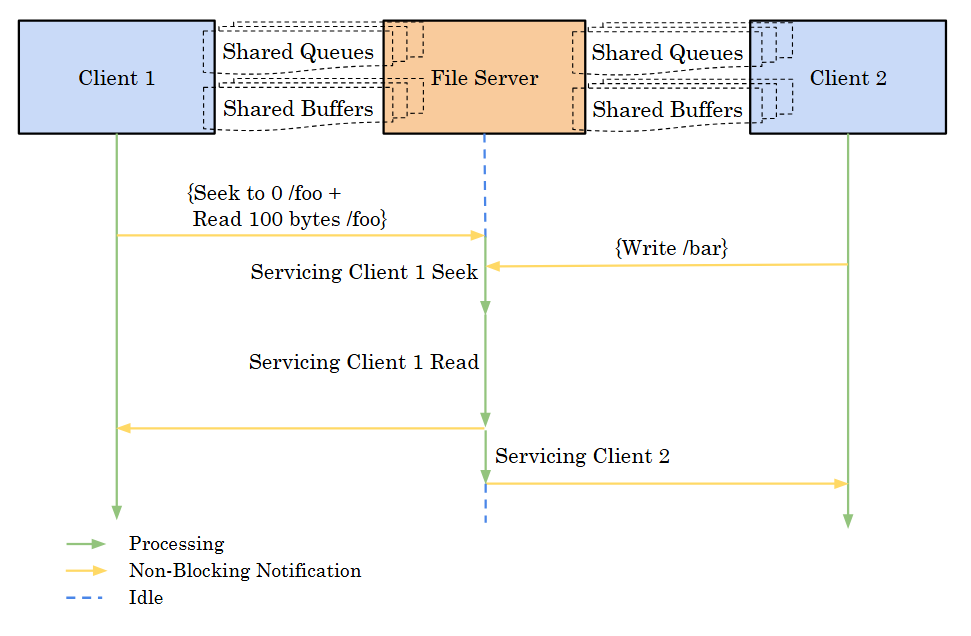
\includegraphics[width=0.68\linewidth]{chapters/images/async.png}
    \caption{Asynchronous multiclient-server interaction.}
    \label{fig:async}
\end{figure} 

While batching can increase the latency of individual operations, it reduces overall IPC frequency and context switching, significantly improving system throughput. Furthermore, the decoupled nature of the interaction allows client execution and server processing to overlap where possible, reducing unnecessary serialization and enabling more efficient utilisation of system resources.

The improvements can be understood through an analytical model of the system. Let $a_n$ denote the time taken for a batch of $n$ operations in the asynchronous system, then let $x$ represent the internal processing time per operation and $c_{a_n}$ represent the communication overhead for the batch.

Therefore, the total execution time for an asynchronous batch of operations can be expressed as:

\begin{equation}
a_n = c_{a_n} + n x
\end{equation}

Hence, the average time per operation is:

\begin{equation}
\frac{a_n}{n} = \frac{c_{a_n}}{n} + x
\end{equation}

This shows that as the batch size increases, the communication overhead is amortised across multiple operations, causing the per-operation communication cost $\frac{c_{a_n}}{n}$ to decrease. In the limit, the average operation time approaches the internal processing cost $x$, indicating that communication overhead becomes negligible.

This highlights the fundamental advantage of batching, as it allows the system to approach a performance bound determined primarily by computation rather than communication.

\section{File Server}

The following subsections discuss the internal design of the file system, including its data structures and organisation. The design focuses on providing a simple and efficient structure to support the required operations, while remaining compatible with both synchronous and asynchronous interface models. 

\subsection{Architectural Overview}

The file server is structured as a set of modular components, each responsible for a distinct aspect of file system operation. Rather than treating the server as a single monolithic body of logic, functionality is decomposed into separate components for request handling, file system operations, runtime state management and storage management. Together, these provide a unified file system service to clients while maintaining clear internal separation of concerns, in keeping with core microkernel design principles.  Furthermore, this modularity supports uniform error handling, allowing failures to be detected accurately, propagated naturally between components and returned to clients in a consistent manner.

At the highest level, the request handling layer forms the entry point into the server, receiving operations from clients and dispatching them to the appropriate file system logic. The file system core implements the semantics of individual file operations, coordinating access to the internal data structures required to service them. Runtime state management maintains transient execution state associated with active file handles, such as access modes and file offsets, while the storage management layer manages the underlying in-memory representation of file contents, metadata and allocation state. This decomposition is illustrated in Figure~\ref{fig:arch}.
\newpage

\begin{figure}[H]
    \centering
    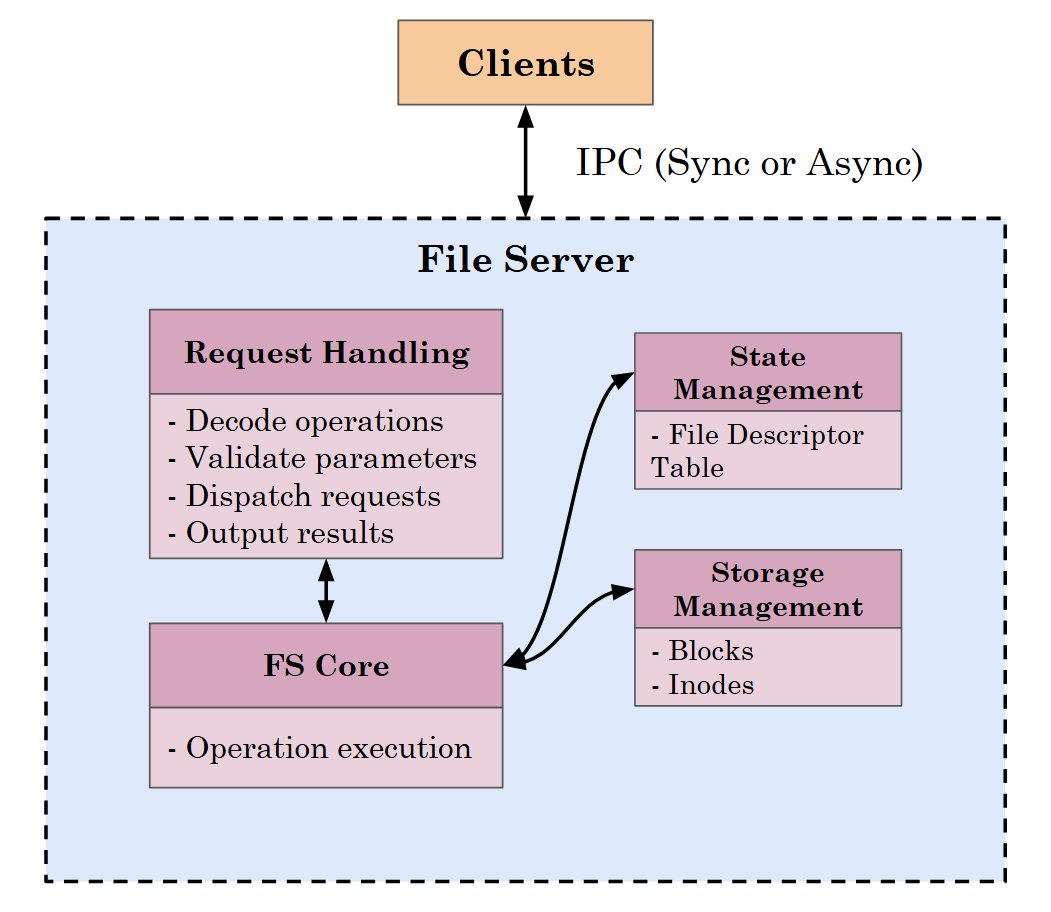
\includegraphics[width=0.55\linewidth]{chapters/images/arch.png}
    \caption{Architectural overview of the file server.}
    \label{fig:arch}
\end{figure}

At a system level, the file server is responsible for servicing client file operations, maintaining correctness of file system state, managing storage resources, and coordinating access across multiple clients. Importantly, these responsibilities are independent of whether requests arrive through the synchronous or asynchronous interface, as both models share the same internal file system logic. This ensures that differences in measured performance arise from interface behaviour rather than differences in core file system operation.

This modular structure allows internal structures or algorithms to be modified without affecting the overall architecture, while supporting extensibility, as features such as persistent storage, more advanced allocation schemes or alternative caching strategies could be introduced without fundamentally redesigning the server.

Hierarchical file storage through a directory structure is supported, allowing files and directories to be organised using path-based naming. Directories may contain both files and subdirectories, enabling nested storage and traversal in a conventional tree-like structure. This was chosen over a flat namespace to support structured organisation and realistic file system behaviour. 

The file server supports a set of operations intended to provide a sufficiently complete and practical file system interface for both functional use and evaluation. These include file and directory creation (Create File, Create Directory), data access (Read, Write, Seek), file lifecycle management (Open, Close, Delete), metadata and state queries (Get Size, Exists, Get Permissions, Set Permissions), and directory enumeration (List).

This set was chosen to provide a balanced interface spanning namespace management, data access, runtime file state and metadata handling. Together, these operations exercise the principal structures and responsibilities of the file server without introducing unnecessary complexity beyond the scope of this work.

\subsection{Component Design and Interactions}

Significant storage management is required to support file system operations, motivating separate structures for representing data, metadata, runtime state and namespace organisation, along with mechanisms to govern their interaction. 

\subsubsection{Blocks}

Blocks form the fundamental unit of data storage in the file server. They represent fixed-size regions of memory used flexibly to hold dynamic file system data, including file contents, directory entries and, where required, block indices for indirect blocks. Using a unified block abstraction allows storage to be allocated according to demand, rather than partitioning memory into separate fixed regions for different data types. This provides greater flexibility, allowing files and directories to grow as required while also avoiding unnecessary reservation of space when demand is low.

A fixed block size was chosen to simplify allocation, indexing and data extension. A size of 4~KiB was selected as a practical balance between storage granularity and management overhead. While fixed-size allocation means all operations occur at block granularity, potentially wasting space when storing very small files, this was accepted in exchange for more efficient allocation management and simpler indexing. As the system is modular, however, this block size remains configurable.

Blocks are managed through an block allocation table, as illustrated in Figure~\ref{fig:bat}. This maintains one entry per block, with each entry storing a flag indicating whether the corresponding block is free or allocated. This enables rapid assignment and release of blocks, simplifying rearrangement of file system data.

\begin{figure}[H]
    \centering
    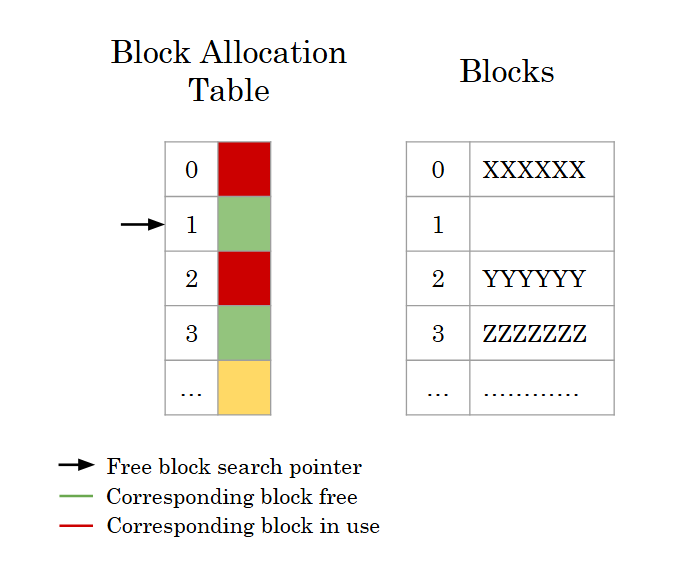
\includegraphics[width=0.55\linewidth]{chapters/images/block_alloc.png}
    \caption{Block allocation table structure.}
    \label{fig:bat}
\end{figure}

All blocks are stored contiguously and are accessed by index into the block pool, with these indices being stored within inodes.

\subsubsection{inodes}

Inodes provide the central metadata structure of the file system, representing either files or directories and linking their logical identity to the underlying storage by holding both entry metadata and block references. This structure was chosen to separate metadata from data storage, simplifying management of file system state. It also provides a uniform representation for file system objects, reducing special-case handling. Furthermore, resolving persistent objects independently of their names avoids repeated path-based lookup. 

\begin{figure}[H]
    \centering
    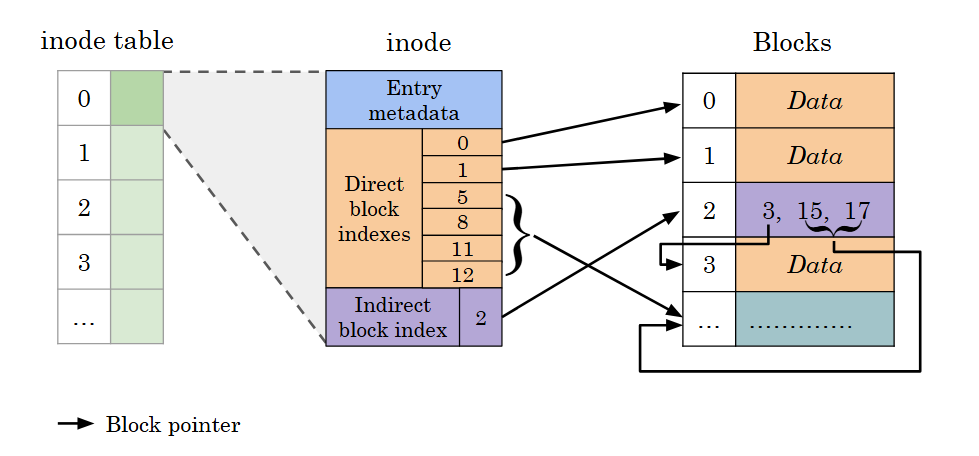
\includegraphics[width=0.8\linewidth]{chapters/images/inode.png}
    \caption{inode and block reference structure.}
    \label{fig:indirect-blocks}
\end{figure}

This metadata must hold a variety of information to allow rich and secure system functionality. To avoid requiring a separate allocation table, each inode includes an in-use flag to enable rapid allocation and deallocation. The inode type (file or directory) is also stored, ensuring associated data is interpreted appropriately and supporting valid file traversal. Ownership and access permissions are additionally stored to support multiple clients safely. 

Inodes store block references either directly or, where additional references are required, through indirect blocks, as shown in Figure~\ref{fig:indirect-blocks}. This allows files to grow beyond the capacity of direct block references while preserving a uniform access model, although very large files may incur modest additional access overhead due to indirect reference resolution. 

To aid efficient data access and ensure only initialised storage is accessed, an inode also stores the file size, indicating the extent of valid file data. Together with the block references, this supports Read operations through resolution of valid file data and Write operations through access to existing blocks, while determining when file extension requires allocation of additional blocks. 

This design introduces an additional level of indirection between file system objects and their underlying data, but this was accepted in exchange for the flexibility, uniformity and scalability the inode structure provides. 

\subsubsection{Directories}

Directories provide the namespace structure of the file system, enabling hierarchical organisation through mappings from names to inode references. They are represented using the same inode and block structures used elsewhere in the file system, reusing existing abstractions rather than requiring a separate storage mechanism, thereby preserving flexibility in data use and storage efficiency. 
\vspace{0.3cm}
\begin{figure}[H]
    \centering
    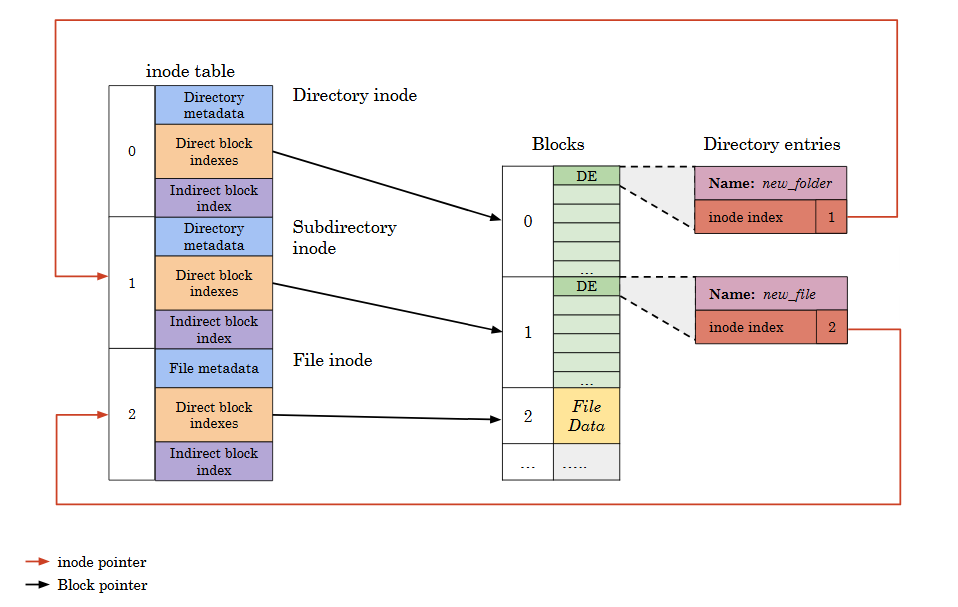
\includegraphics[width=0.9\linewidth]{chapters/images/dir_inode.png}
    \caption{Directory structure via inodes and blocks.}
    \label{fig:directory-entries}
\end{figure}

A directory is represented by a directory inode whose associated blocks store a list of nested files and subdirectories as directory entries. Each directory entry is a structure linking an entry name to its respective inode via an index, as shown in Figure~\ref{fig:directory-entries}. 
\newpage
This recursive structure enables hierarchical namespace organisation through arbitrary nesting of directories and files, supporting structured management beyond what would be possible in a flat namespace. It also provides inherent path-based access, where successive path segments are resolved by searching the entries of the current directory, descending into a child directory when a matching entry is found, until the target inode is reached, or a path is deemed invalid. This traversal mechanism is used by file system operations to inspect and modify directory entries, enabling Create to enforce valid paths and prevent duplicate names within a directory, while supporting recursive directory deletion through traversal of all contained entries to ensure no unreachable data is left allocated. 

For general use, a root directory is created during system initialisation, through which all files and directories are organised upon, hence, may not be deleted. Special directory entries such as . and .., as well as symbolic links, are not supported, reducing namespace complexity and avoiding additional traversal cases. 

This structure was chosen to support path-based access and structured file lookup, allowing files to be located through traversal rather than requiring a flat naming model. However, as path resolution requires directory traversal, lookup incurs some overhead, particularly due to linear directory scans and possibly deeply nested paths. Linear scanning was chosen over more complex indexed lookup structures to reduce management overhead and implementation complexity, which was considered appropriate for the expected scale of the file system, while not affecting comparisons of the synchronous and asynchronous communication models. 

\subsubsection{File Descriptors}

File descriptors maintain runtime state for open files, providing a layer of indirection between client operations and persistent file metadata. As shown in Figure~\ref{fig:file-descriptors}, a file descriptor links a client-visible handle to the inode representing the underlying file, while additionally storing the transient state required for continued access.

\begin{figure}[H]
    \centering
    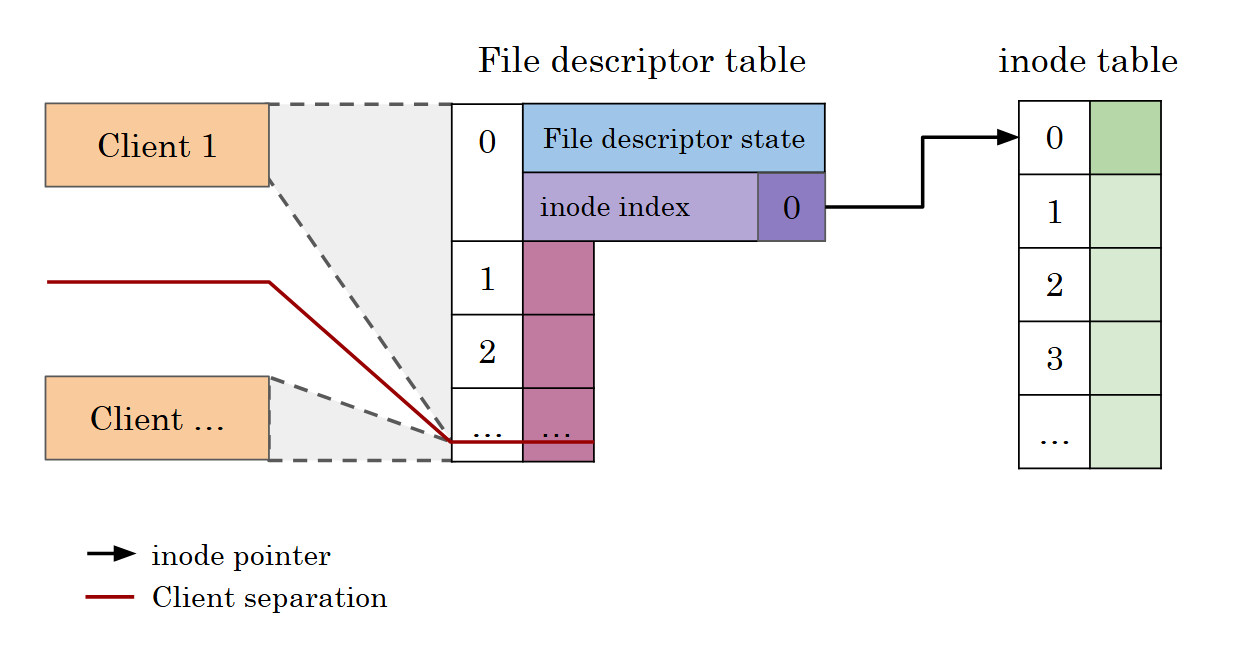
\includegraphics[width=0.7\linewidth]{chapters/images/fds.png}
    \caption{File descriptor structure.}
    \label{fig:file-descriptors}
\end{figure}
\newpage

This state includes a reference to the associated inode, the current file offset, and the mode in which the file was opened. Separating this runtime state from inode metadata allows information specific to an active open instance, rather than the file itself, to be maintained, supporting multiclient access. This is additionally useful for operations such as sequential reads or writes, where file position may persist across operations and need not be re-specified.

File descriptors are created and returned to a client when a file is opened, and are subsequently used by operations such as Read, Write, Seek and Close to reference the open file. This improves efficiency by avoiding path resolution for every operation, as the file descriptor is used to link directly to the associated inode.

This design does introduce some overhead in maintaining descriptor state, but this is modest relative to the performance benefits it provides. Fixed-size file descriptor regions do, however, impose a bounded number of simultaneously open files per client.

\subsection{Request Processing Flow}

File system requests follow a common processing path regardless of operation type. Once a request is received by the file server, it is first decoded to determine the requested operation and extract any associated parameters. Basic validation is then performed, such as verifying the operation code is recognised, the required parameters are present and checking that any referenced file handles or paths are correctly formed.

Following validation, the request is dispatched to the appropriate file system logic. Although the specific structures accessed differ by operation, all requests follow the same general pattern of interacting with the file system core, consulting or updating the relevant runtime state, accessing the underlying storage structures as required, and generating a result to return to the client.

The general flow is:
\begin{itemize}
    \item Receive request
    \item Decode operation
    \item Validate parameters
    \item Service operation
    \item Access internal structures
    \item Update state if required
    \item Generate response
\end{itemize}

For example, Read request follows this general structure by validating the supplied file handle exists and is a file, consulting the open file state to determine the current offset, resolving the relevant storage blocks containing the requested data, and returning the result while updating the file offset. Operations such as Create and Write access and modify different state, but follow the same overall dispatch and servicing model.

This shared processing path was chosen to reduce duplicated logic, ensure consistent validation across operations, and simplify reasoning about correctness within the file server.

\subsection{Multiclient Support}

Multiclient support is provided through a combination of per-client runtime state, client isolation and centralised coordination through the file server. This allows multiple clients to access the file system concurrently while preserving correct behaviour and separation of client context.

Per-client state is maintained through both persistent and runtime structures. Ownership and access permissions are stored within inode metadata, allowing access control decisions to be enforced consistently regardless of which client issues a request. Permissions are represented using read, write and execute flags, allowing the file server to determine whether a client may perform a requested operation. Ownership associates each file or directory with the client that created it and restricts operations such as permission modification. Ownership also supports private access: if a permission flag is unset, only the owner may perform the corresponding operation, whereas if the flag is set, any client may do so. 

Runtime state associated with open files, such as file offsets and access modes, is maintained in file descriptors. To preserve client independence, each client is assigned a separate region of the file descriptor table, with a local maximum number of open files. This ensures that one client’s open file state cannot interfere with that of another. This separation of runtime state provides client isolation even when multiple clients access shared resources. While multiple clients may access the same underlying file, each does so through its own client context, maintaining independent offsets, access modes and descriptor state.

Consistency of shared resources is preserved through centralised mediation by the file server; all file operations pass through the server and are serviced atomically, with updates to shared file system structures serialised. 

A particular case of shared resource consistency arises when one client deletes a file that remains open by others. In this case, deletion is deferred until the final client closes the file, ensuring that active references remain valid and preventing removal of data still in use.

